\documentclass{article}

\usepackage[export]{adjustbox}
\usepackage{listings}
\usepackage{subcaption}
\usepackage{wrapfig}
\usepackage[dvipsnames]{xcolor}
\usepackage{float}
\usepackage{graphicx}
\usepackage[export]{adjustbox}
\usepackage[utf8]{inputenc}
\usepackage[a4paper, top=4cm, bottom=4cm, left=4cm, right=4cm]{geometry}

\title{
    \textbf{\textit{SafeStreets}} \\
    \textbf{DD document}}

\date{Academic year: 2019 - 2020}
\author{
    Dario Miceli Pranio \\
    Pierriccardo Olivieri
}

\begin{document}
\pagenumbering{gobble}

\maketitle

%%%%%%%%%% LOGO POLIMI %%%%%%%%%%
\begin{figure}[h!]
    \centering
    
\includegraphics[scale=0.5]{img/logo.png}
\end{figure}

\newpage
\pagenumbering{arabic}
\tableofcontents

\newpage
%%%%%%%%%% CHAPTER 1 %%%%%%%%%%
\section{Introduction}

\subsection{Purpose}
The purpose of this document is to provide a functional description of \textit{SafeStreets} application.

\subsection{Scope}
\textit{SafeStreets} is a service that aims to provide \textit{Users} with the possibility to notify \textit{Authorities} when traffic 
violations occur, and in particular parking violations. The application's goal is achieved by allowing \textit{Users} 
to share photo, position, date, time and type of violation and by enabling \textit{Authorities} to request them.
\\
\\
\textit{SafeStreets} requires the \textit{Users} to create an account to access its services, the functionalities unlocked after 
registration depend on the type of account created.
\\
If a \textit{User} creates an account as \textit{Citizen}, he/she must provide name, surname and a fiscal code in order to prove 
that he/she is a real person. Furthermore, he must provide an email with which he will be uniquely identified 
and a password. Once the account has been activated, \textit{User} can finally start to report parking violations and can also see 
statistics of the streets or the areas with the highest frequency of violations.
\\
\\
On the other hand, an officer will create an account as \textit{Authority} and he will need to provide his name, surname, 
work's Matricola, a password and as for \textit{Citizen}, will be uniquely identified by an email. Once the Matricola 
has been verified and the account has been activated, the officer can retrieve the potential parking violations 
sent by \textit{Citizen} that have not been taken into account yet by other officers, analyze them and, if it is the 
right case, generates traffic tickets. \textit{Authorities}, can see the same statistics of the \textit{Citizen} and can also see
statistics about vehicles' license plate that commit the most violations.


\subsection{Definitions, acronyms, abbreviations}

\subsubsection{Definitions}
\begin{itemize}
    \item \textit{Users}: can be either \textit{Citizen} or \textit{Authority}
    \item \textit{traffic violation}: generic violation that can occur in a street
    \item \textit{parking violation}: a violation caused by a bad parking
    \item \textit{violation}: general violation, identity both traffic or parking violation
    \item \textit{unsafe areas}: areas with an high rate of violations
    \item \textit{Driver}: a piece of software that simulates a component that depends on the module undergoing testing
    \item \textit{Stub}: a piece of software that simulates a components on which the module undergoing testing depends
    \item \textit{Client}: Software \textit{System} on the \textit{User's} device that requests services to the Server
    \item \textit{Server}: Software \textit{System} that handles requests from different clients
    \item \textit{n-tier}: Distributed architecture composed of n hardware components, each containing one or many layers
    \item \textit{n-layer}: Distributed architecture composed of n software levels, each distributed on one or many tiers.
    \item \textit{Design}: Pattern: Reusable software solution to a commonly occurring problem within a given context of software design.
\end{itemize}

\subsubsection{Acronyms}
Table with all acronyms used in document.
\begin{center}
\begin{tabular}{ | l | l |}
    \hline
    ACRONYM & COMPLETE NAME \\
    \hline
    DD & Design Document \\
    \hline
    RASD & Requirements Analysis and Specification Document \\
    \hline
    GPS & Global Positioning Systems \\
    \hline
    S2B & Software To Be \\
    \hline
    STNP & Simple Time Network Protocol \\
    \hline 
    FC & Fiscal Code \\
    \hline
    DB & Database \\
    \hline
    ORM & Object-Relational Mapping \\
    \hline
    MVC & Model View Controller \\
    \hline
    DBMS & Database Management System \\
    \hline
    REST & REpresentational State Transfer \\
    \hline
    UI & User Interface \\
    \hline
    UX & User Experience \\
    \hline
    HTTP & HyperText Transfer Protocols \\
    \hline
\end{tabular}
\end{center}

\subsubsection{Abbreviations}
\begin{itemize}
    \item \textbf{Rn}: n-th Requirement 
\end{itemize}

\subsection{Revision History}
\begin{center}
    \begin{tabular}{ | l | l |}
        \hline
        VERSION & CHANGES \\
        \hline
        1 & First release \\
        \hline
        1.1 & Minor change on image \\
            & Error correction \\
        \hline
    \end{tabular}
    \end{center}

\subsection{Reference documents}
\begin{itemize}
    \item ISO/IEC/IEEE 29148: https://www.iso.org/standard/45171.html
    \item Specification Document: "SafeStreets Mandatory Project Assignement"
\end{itemize}

\subsection{Document Structure}
This section is a guide through the document, a short explanation on what we will discuss.
\begin{itemize}
    \item \textbf{Chapter 2: Architectural Design}\\
    In this chapter, starting from an informal overview, is described deeply the \textit{System}
    architecture, with the use of components diagrams and component interface diagrams. It is also
    described using sequence diagrams how \textit{System} behave in a runtime perspective.

    \item \textbf{Chapter 3: User Interface Design}\\
    As already described in the RASD document with mockups, in this section is analyzed the 
    UI flow that shows how those mockups interact in a dynamic context.

    \item \textbf{Chapter 4: Requirements Traceability}\\
    This chapter is focused on the relation between the requirements from the RASD and
    the design choices of the DD.

    \item \textbf{Chapter 5: Implementation, Integration and Test Plan}\\
    Explain the implementation for \textit{SafeStreets} application and how it is 
    tested, the integration of all component and how is organized the testing phase.

    \item \textbf{Chapter 6: Effort Spent}\\
    A table where is described the effort spent for each group member for this project.

\end{itemize}

%%%%%%%%%% !CHAPTER 1 %%%%%%%%%%

\clearpage

%%%%%%%%%% CHAPTER 2 %%%%%%%%%%
\section{Architectural Design}

\subsection{Overview: High level components and their interaction}

\begin{figure}[H]
    \centering
    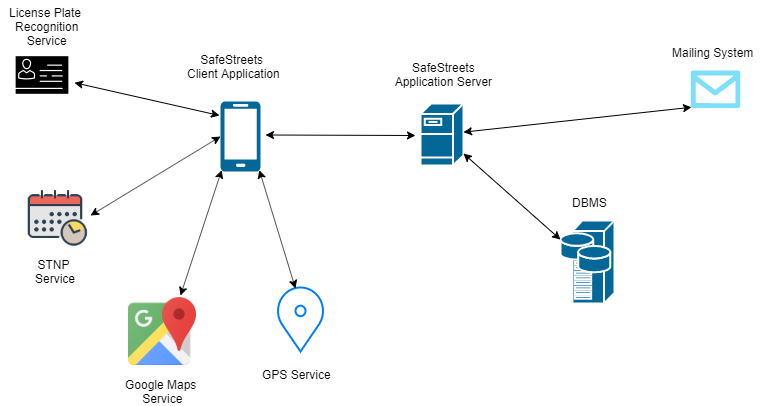
\includegraphics[scale=0.3]{img/overview.png}
    \caption{\textit{System's} Overview}
\end{figure}

In this graphical representation of \textit{SafeStreets} we describe at an high level the main interaction
between the components that are involved. Focusing on client side \textit{SafeStreets} provides a Client 
application, in this view case we don't make a distinciton between the \textit{Users} type, this is 
primarily devoted to the fact that the requests are similar. We identify then a 3-tier architecture, 
composed by the client, a proxy in the middle to manage properly all the requests and finally a back 
end part in which the \textit{System} store the information (in a DBMS) and generate statistics thanks
to the data submitted by the \textit{Citizen} and confirmed by \textit{Authorities}. In order to do this
we need an application server. Since we will authenticate the \textit{Users} through a confirmation email, 
and we give the possibility to the \textit{Authority} to receive data via mail, the \textit{System} needs
also a Mailing System. Finally we also need some service in the client like GPS Service, Maps Service,
STNP Service and License Plate Recognition Service. These services are essential to create a proper violation
and to send it correctly.

\clearpage
\subsection{Component view}
\textbf{Component High Level View} \\
The following 3 images will show at an high level how the \textit{System} is organized, as we can see the
choice we made is a classic client-server architecture. 

\begin{figure}[H]
    \centering
    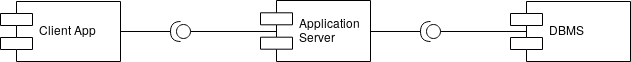
\includegraphics[scale=0.4]{img/component_diagrams/component_diagram.png}
    \caption{Component Diagram High Level View}
\end{figure}
The client presents various components 
each one covering a different role: the Presentation Manager that corresponds to the “View” in the MVC Pattern 
is the medium between the application and the \textit{User}, Logic Manager is the component designed to catch 
all the application Logic, it orchestrates the send report action for \textit{Citizens} and the retrieve report 
action for \textit{Authorities}, Logic Manager is also connected to a cache storage in order to save momentaneously 
data. The Security Manager, crucial for the application, is the component used to ensure the message security 
during the trasmission to server, his main job is to apply a digital signature. The Network Manager handles the
connection and is the component that communicates with server.

\begin{figure}[H]
    \centering
    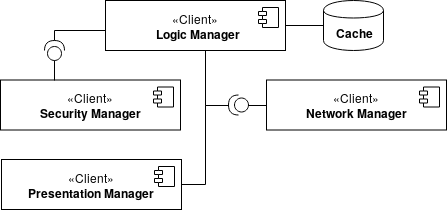
\includegraphics[scale=0.6]{img/component_diagrams/client_component.png}
    \caption{Client view}
\end{figure}

The server presents the Network Manager for communication, and various components for \textit{SafeStreets}'s main actions
like report, statistics and settings that are embedded in the Report Manager, Statistics Manager and Settings
Manager respectively. To handle all the auth operations we will use the Authentication Manager, that with the 
help of Privacy Manager will authenticate an \textit{User} in order to give access to actions. All this components needs 
to communicate with database in order to store permanently or modify data, and this is possible thanks to 
the Database Manager, infact database is system-independent, and all the communications pass through this 
component. The Statistics Manager has also a cache in which can store the generated statistics to send to the
requestor, this is a way to reduce database access and to fulfill the request in a rapid way.  
\begin{figure}[H]
    \centering
    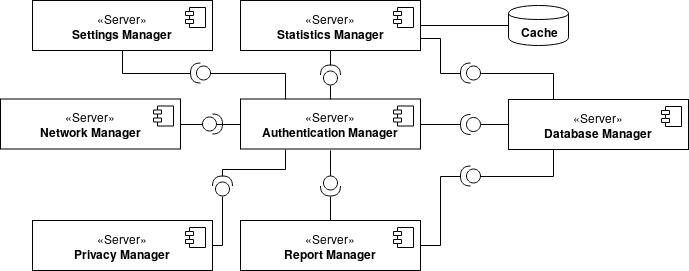
\includegraphics[scale=0.6]{img/component_diagrams/server_component.png}
    \caption{Server view}
\end{figure}
\textbf{Component View}\\
Here we go deeper in the Component Diagram, are described all the interactions between the component
described above and all the external services like the Maps service, license plate Recognition Service and 
STNP service for the client and Mailing System for the server.

\begin{figure}[H]
    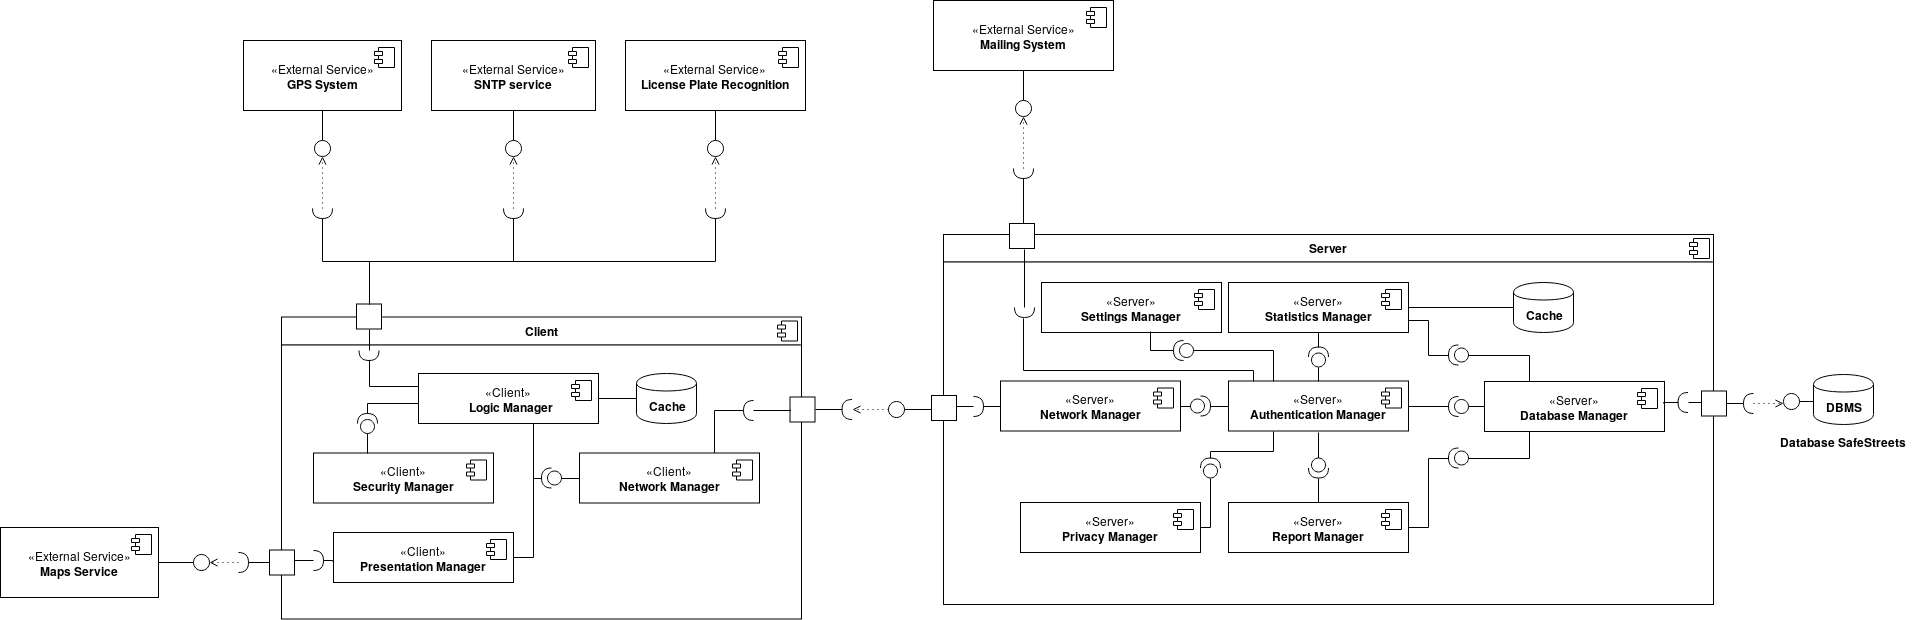
\includegraphics[width=1.2\textwidth, left]{img/component_diagrams/component_diagram_complete.png}
    \caption{Component Diagram Detailed view}
\end{figure}

The purpose of this UML diagram is to show the internal architecture of the \textit{System}'s software. It's divided in 
three component: \textit{SafeStreets} Client Application, \textit{SafeStreets}'s Server, External interfaces.
Below we will describe each component.
\\
\\
\textbf{Network Manager}: \\
The network manager is the component designed to manage the sending and receiving of 
messages exchanged between client and server, it is located both in the client and in the 
server, this component also has the task of correctly routing the messages to the correct 
component.
\\
\\
\textbf{Client}:

\begin{itemize}

\item \textbf{Presentation Manager}:\\
This client side component is the main intermediary between \textit{User} and \textit{SafeStreets}. 
Interface management is totally entrusted to this component, in terms of scalability it 
is advantageous to separate the interface from the rest of the application. Encapsulating 
everything in the Presentation Manager will be helpfull to reduce problems whether in future 
will be necessary to change part of the interface or to develope the client for a new type of 
operating system.

\item \textbf{Security Manager}:\\
Security in report transmission is critical. Separating security techniques into a 
separate component \textit{SafeStreets} can ensure greater scalability in terms of security 
by implementing the best methods. The component currently deals with the digital signature 
of the report before sending and also checking the validity of the digital signature of a 
report.

\item \textbf{Logic Manager}: \\
This is the main component of the client, it communicates with the presentation manager, 
security manager, network manager and with all the external services, it is the central 
unit of the Client. The purpose of this component is to perform all the operations that 
the \textit{User} requires through an interface such as report sending operations (\textit{Citizen}) 
or request report (\textit{Authority}) but also the statistics request and the edit settings. 
The first two (send and receive report) operations are very important, the Logic Manager 
is therefore connected to a cache that has multiple uses, in the case of the {Citizen} this 
cache is used to temporarily save the report, this step is necessary because if the \textit{User} 
sends the report and this is subjected to a malicious attack the server will notice upon 
arrival that the digital signature does not match, discarding that report. To avoid loosing it, 
the Logic Manager saves it in the cache and sends it periodically until the confirmation is 
received. The Logic manager also deals with the creation of the report, carrying out all the 
necessary operations, collecting data from external services, executing the license plate 
recognition algorithm and using the services of the Security Manager to apply the digital 
signature to the report to guarantee its security in the way to server, in the same 
way for the report retrieval function, with the help of the Security Manager, the validity of 
the digital signature will be checked. 
\end{itemize}

\textbf{Server}:

\begin{itemize}

\item \textbf{Database Manager}: \\
The database access intermediary resides in this component, every access to the database in 
fact passes through the Database Manager, this brings advantages in scalability and flexibility 
since it makes the server independent from the database. Among the various operations it deals 
with the authentication of the \textit{User}, therefore the operations of login and registration, 
of statistics retrieval and report insertion or retrieval. This component will use an 
ORM in order to abstract the implementation details of the Database.

\item \textbf{Authentication Manager}: \\
This component is of fundamental importance on the server side, not only does it takes care 
of all the login and \textit{User} registration procedures, it is also the access port for which all 
the other components must pass in order to execute their procedures, in fact no component 
can perform an operation coming from a request from an unauthenticated \textit{User}.

\item \textbf{Privacy Manager}: \\
This component deals with the security of \textit{User's} sensitive data, especially passwords 
and personal data must be encrypted before being inserted into the database, for greater 
flexibility and any changes it was preferred to separate that component. 
It communicates exclusively with the Authentication Manager and has the task 
of check the hash of the password stored in the DB with the hash of the 
password sent by the client.

\item \textbf{Settings Manager}: \\
The \textit{User} may want to change his data, update the email or name and surname. To do this, these 
requests, on the server side, are forwarded to the Settings Manager which communicates directly 
with Authentication Manager and Database Manager to ensure the success of the action. 

\item \textbf{Statistics Manager}: \\
The statistics of the application are generated at time intervals, in fact does 
not make sense to constantly update them, since statistics can only be changed by an \textit{Authority} that
check a report, so it can be considered as a slow process. This component then takes care of creation 
of the statistics and saves them in the appropriate cache where they are updated periodically. 
The Statistics Manager generates all types of statistics for both Violations and Vehicle and 
forwards the most updated from the cache to the Client when requested.

\item \textbf{Report Manager}: \\
The Report Manager takes care of the two key functions of \textit{SafeStreets}. The send report and 
the retrieve report, in fact by communicating with the database through the Database Manager 
it can save the incoming reports or manage the sending of those that should be evaluated. 
It also deals with the security logic, in fact if the report received does not correspond 
with the digital signature this will be immediately discarded. When a report is evaluated 
by an \textit{Authority}, this component will take care of updating the respective report and 
notifying the Statistics Manager.
\end{itemize}

\clearpage
\textbf{External interfaces} \\
Some of the described components in our \textit{System} are also dedicated to communicating 
with external services through specific interfaces. It is essential that the communication 
works properly in order to fulfill application's functionalities.
This external services are:
\begin{itemize}
    \item Database \\
    The component devoted to interacting with the central database on 
    cloud is the Database Manager.
    \item GPS \\
    On the Client side of the application, \textit{SafeStreets} access data from 
    the \textit{User}'s device's GPS. GPS information are important because are used in 
    report to locate a position. 
    \item Mailing System \\
    It used by Authentication Manager to inform an \textit{User} that his account 
    has been correctly created. 
    \item Maps Service \\ 
    It's used to show unsafe areas in statistics.  
    \item STNP service \\
    It is used to retrieve the correct Time and Date to attach to reports.
    \item License Plate Recognition Service \\
    This service taking in input the violantion's photo will try to recognize the license plate.
\end{itemize} 

\clearpage

\subsection{Deployement view}
\begin{figure}[H]
    \centering
    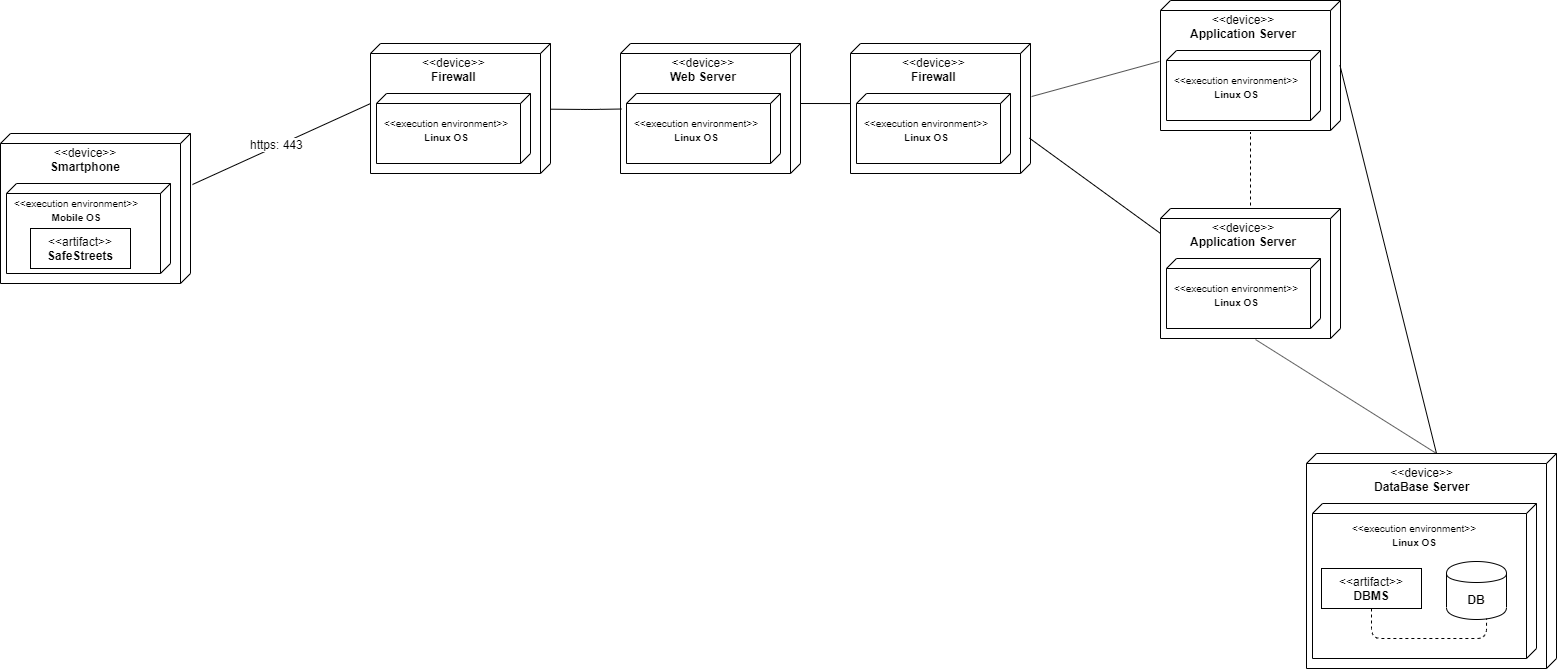
\includegraphics[scale=0.3]{img/Deployment_component.png}
    \caption{Deployment view}
\end{figure}  
The architecture choosed for \textit{SafeStreets} is a multi-tier architecture. Below all the nodes 
involved will be described.
\\
\\
\textbf{Smarthphone}\\
Represents the \textit{User's} smarthphone in which the client will run. This is the client machine
that will run \textit{SafeStreets} application.
\\
\\
\textbf{Firewall}\\
Necessary to provide protection between local network and world network, so not-allowed third 
parties will not be able to access data. In particular we decided to use two firewalls to create a DMZ. 
The first firewall must be configured to allow traffic destined to the DMZ only. The second firewall 
only allows traffic to the DMZ from the internal network.
\\
\\
\textbf{Application Server}\\
Is the central unit of \textit{SafeStreet} all the other components refer to this. It 
contains all the logic and provide bidirectional access to Database i.e. manages data 
acquisition and requests. We decided to fully replicate Application Servers in order 
to balance the workload and to avoid denial of service.
\\
\\
\textbf{Proxy}\\
\textit{System} will use a proxy to receive requests. This solution is more scalable 
for the eventuality of further improvements and guarantee a better stability of 
the \textit{System}. Furthermore Proxy acts as additional shield against security attacks.  
\\
\\
\textbf{Database}\\
A Database is necessary in order to store all the informations about personal data, 
registration and data submitted by \textit{Citizen} and retrieve information in order, 
for instance, to build statistics.

\clearpage

\subsection{Runtime View}
\textbf{Proxy Runtime View}\\
The following sequence diagram describes how the Proxy interacts with the Client and the Application 
Server. When an \textit{User} sends a request, checks whether such request conforms to its defined schema and, 
in case the \textit{User} has to be logged in, checks if the provided authToken is associated to an actual 
logged in \textit{User}. This last check, in particular, is efficient to be done on the Proxy instead of each 
Application Server, because if a \textit{User} logs in with a particular Server which then crashes, the 
\textit{User} doesn't have to log in again, since the information is stored on the Proxy. In this sequence diagram
the function "sendRequest(req)" is a generic call that represents one of the possible client's actions.

\begin{figure}[H]
    \centering
    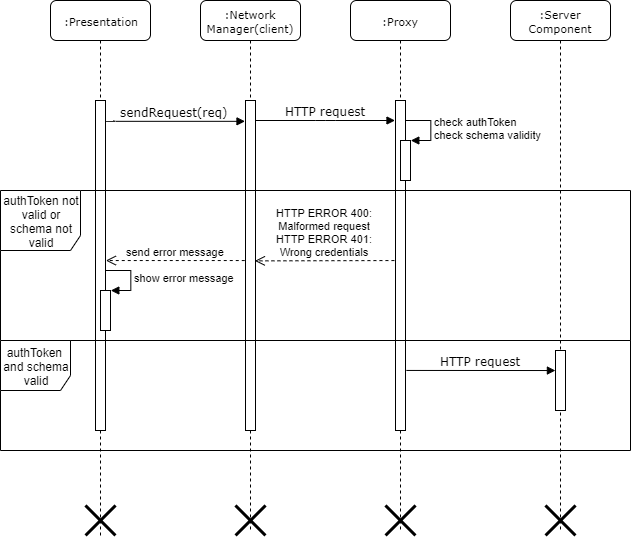
\includegraphics[scale=0.4]{img/sequence_diagrams/Proxy_sequence.png}
    \caption{Proxy Runtime View}
\end{figure}  
\clearpage
\textbf{Login Runtime View}\\
The following diagram describes the sequence of events when a \textit{User} tries to login in 
\textit{SafeStreets} application. The actors involved are the Presentation, Logic and the Network Manager on the
client and the Network Manager, Authentication Manager and the Database Manager on the Server.
When a \textit{User} wants to login in his account, an HTTP request is sent to the application Server
containing his credentials. Database Manager checks the validity of credentials by quering DB. If the query
success then \textit{User} can correctly be authenticated. The two errors that can occur are HTTP ERROR 400:
Malformed Request and HTTP ERROR 401: Wrong Credentials. The first one occurs when request's format is invalid,
such as having empty parameters. The second one occurs when credentials are wrong.   

\begin{figure}[H]
    \centering
    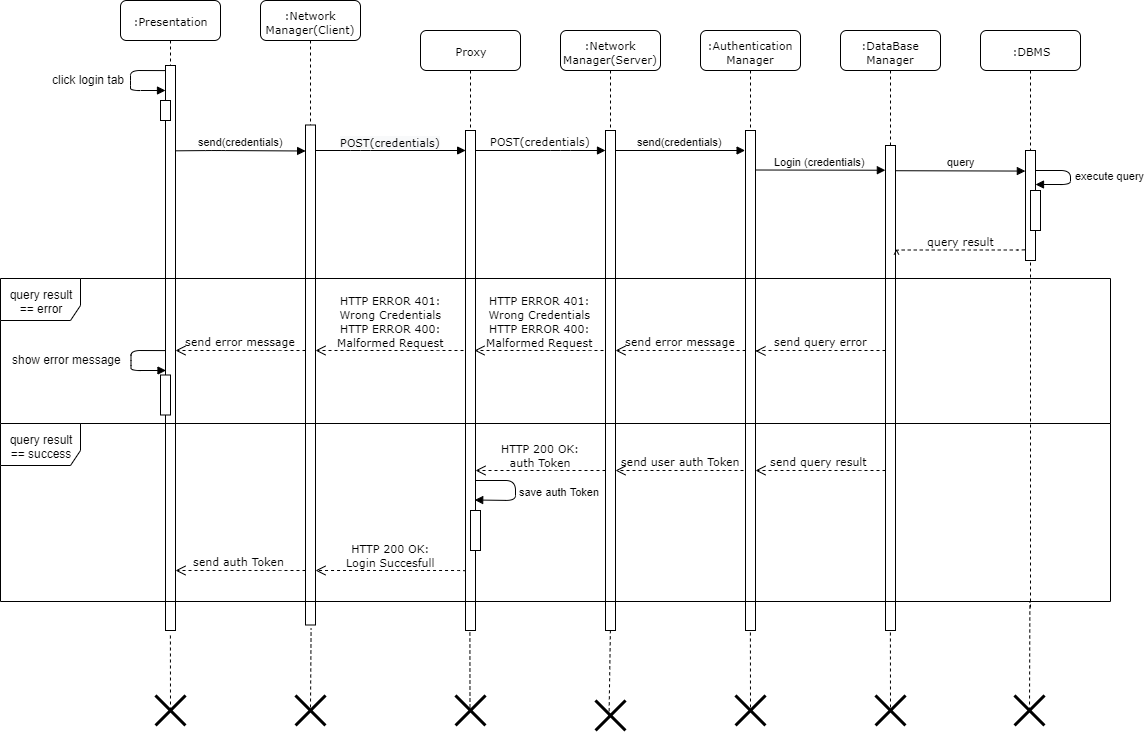
\includegraphics[scale=0.3]{img/sequence_diagrams/login_sequence.png}
    \caption{Login Runtime View}
\end{figure}  

\clearpage
\textbf{Registration Runtime View}\\
The registration sequence shows the step followed for the 
registration of a new \textit{User}. The two registration procedures for \textit{Citizen} and  
\textit{Authority} are similar, the only thing that change is the code used, for the first is 
needed the fiscal code for the second the Matricola number. To avoid a duplicate we show here 
the general procedure. After filling the form data is sended through the proxy to the server, 
here data will be secured and stored in the database. Here two situations may occur, the \textit{User} 
data aren't already present in the database so \textit{User's} data will be stored and \textit{System} 
can continue with the process sending client a success message or data inserted have been already used 
by another \textit{User} and the client will receive an error message. This process will be repeated 
until success message. When \textit{User's} data are correctly stored the \textit{System} will send a 
confirmation email with a token in order to activate the account. Then \textit{System} waits until the 
\textit{User} clicks the confirm link in the mail received, clicking the link will send the token to 
server, again two situation may occur, the token is valid and the procedure terminate with the account 
activation or the token isn't valid and the \textit{User} needs to request another confirmation email.

\begin{figure}[H]
    \centering
    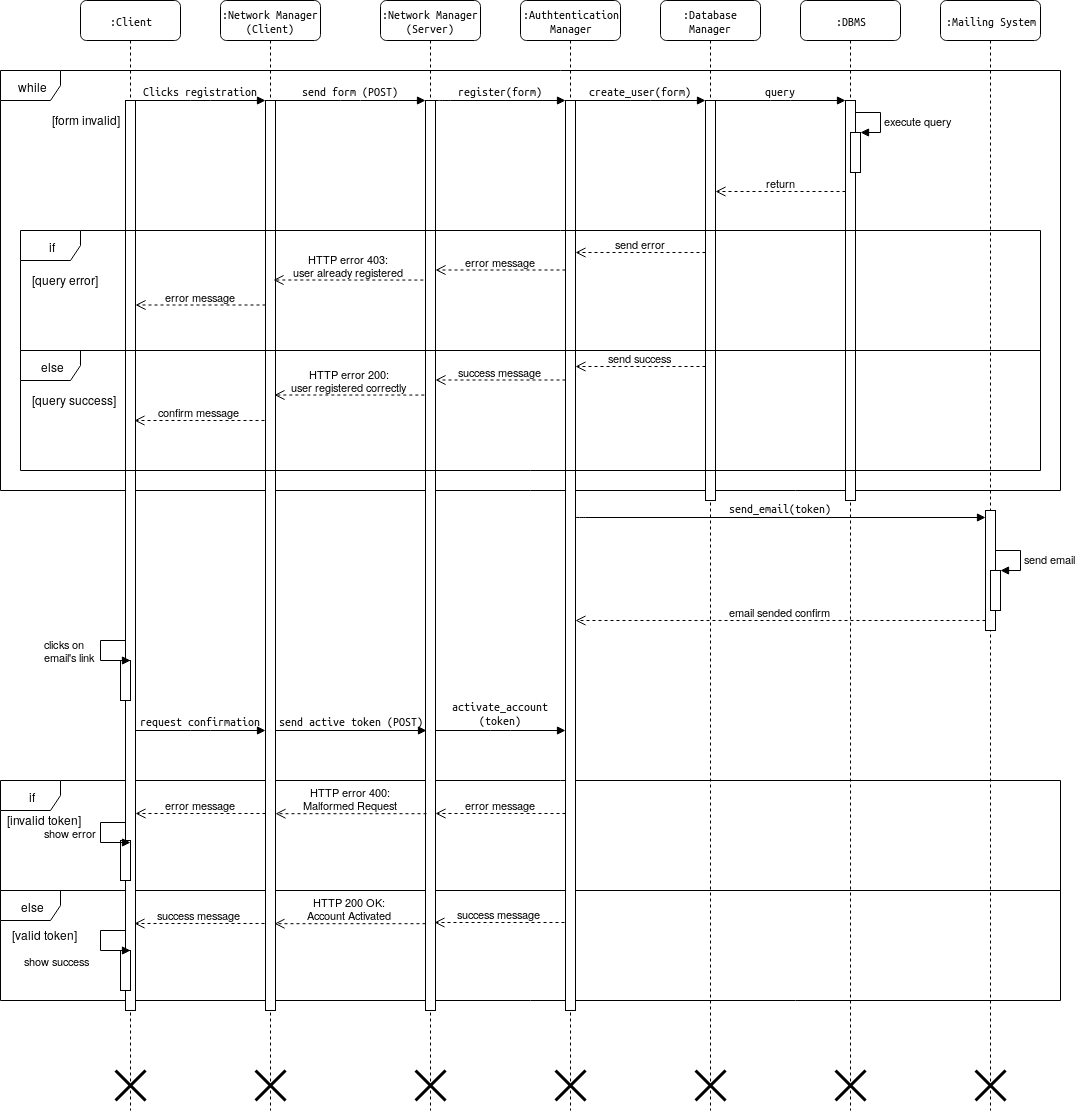
\includegraphics[scale=0.3]{img/sequence_diagrams/registration_sequence.png}
    \caption{Registration Runtime View}
\end{figure}  
\clearpage
\textbf{Send Report Runtime View}\\
The following diagram represents the sequence of actions executed on the \textit{Citizen's} send report, 
first all the necessary data is gathered, the next sequence will describe in a more detailed way how it's 
done, here is simplified for a better readability. Then data collected is passed at the Logic Manager, 
it will secure the data applying a digital signature through the Security Manager, then the violation is 
saved momentaneously in the cache and sent to the server. As described in the picture, Logic Manager 
saves the violation in the cache to avoid loss, if there is a malicious attack in the way to the server, 
in order to modify the violation, then the digital signature will be compromised, in this case the server 
will reject the violation and it will be lost. To avoid this inconvenience the client saves the report 
in the cache and will send it at every timetout until it recevies from the server the success message. 
In the other hand the server will save the report and send the success message if only if the digital 
firm is correct. 

\begin{figure}[H]
    \centering
    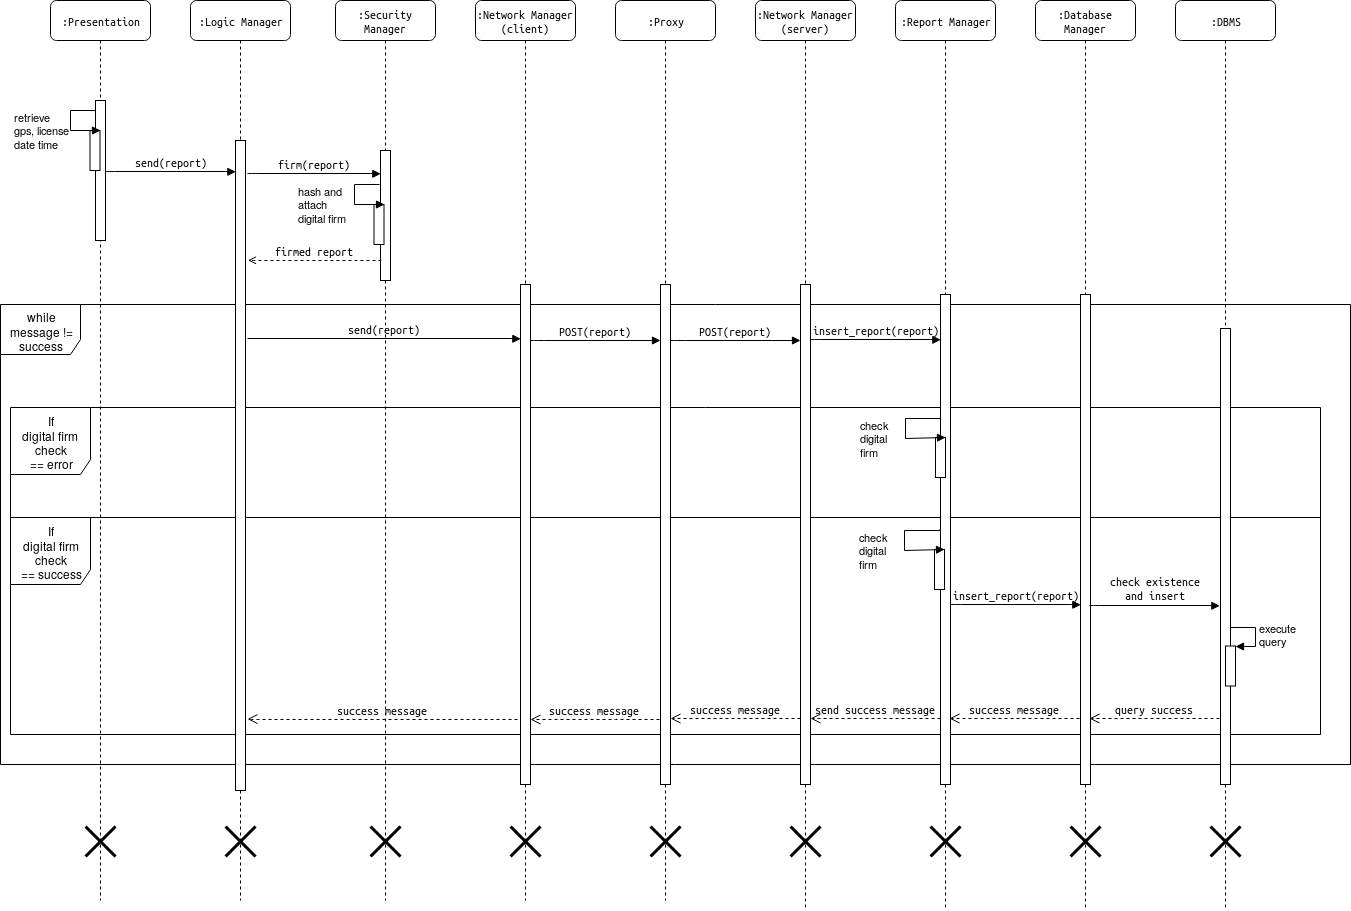
\includegraphics[scale=0.3]{img/sequence_diagrams/send_report_sequence.png}
    \caption{Send Report Runtime View}
\end{figure}  
\clearpage
\textbf{Collect External Data Runtime View}\\  
This is a "zoom" on the self call "retrieve gps, license, date time" that Presentation does in the 
previuos sequence, it's only a graphical semplification in aim to better understanding the process, 
separating this fase make more readable the previous image. These steps show how information are 
retrieved from external services, those information will be used to create the report by the Logic Manager.
\\
\\
\begin{figure}[H]
    \centering
    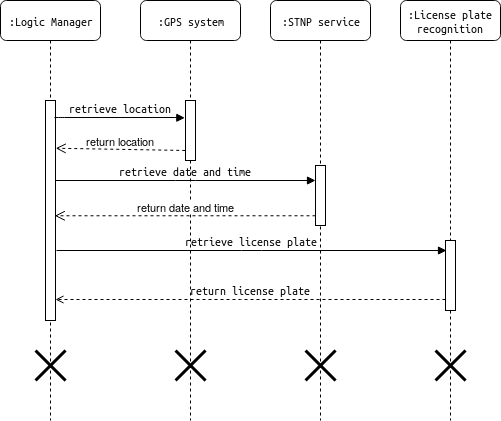
\includegraphics[scale=0.6]{img/sequence_diagrams/collect_external_data_sequence.png}
    \caption{Collect External Data Runtime View}
\end{figure}
\clearpage
\textbf{Retrieve Report Runtime View}\\
The following diagram describes the sequence of events when an \textit{Authority} tries to retrieve a violation in
\textit{SafeStreets} application. The actors involved are the Presentation, Logic Manager, Security Manager and 
the Network Manager on the client and the Network Manager, Report Manager and the Database Manager on the Server.
When an \textit{Authority} clicks the retrive button an HTTP request is sent to the Application Server in order to
query the DB and retrive the violation. Once the violation has been retrieved, Security Manager checks violation's 
validity by computing the hash and matching it with the one from the digital signature. If the two hash are the same then
Security Manager sends the violation to \textit{Authority}. When \textit{Authority} clicks the "YES" or "NO" button a final
HTTP request is sent to Application Server containing the response. It is important because in this way \textit{System} can
build Statistics. If, instead, the two hash are not the same then a malicious attacker is trying to alterate information so
Logic Manager discards the violation and waits for the timeout. In this way Report Manager can sends the violation again.     

\begin{figure}[H]
    \centering
    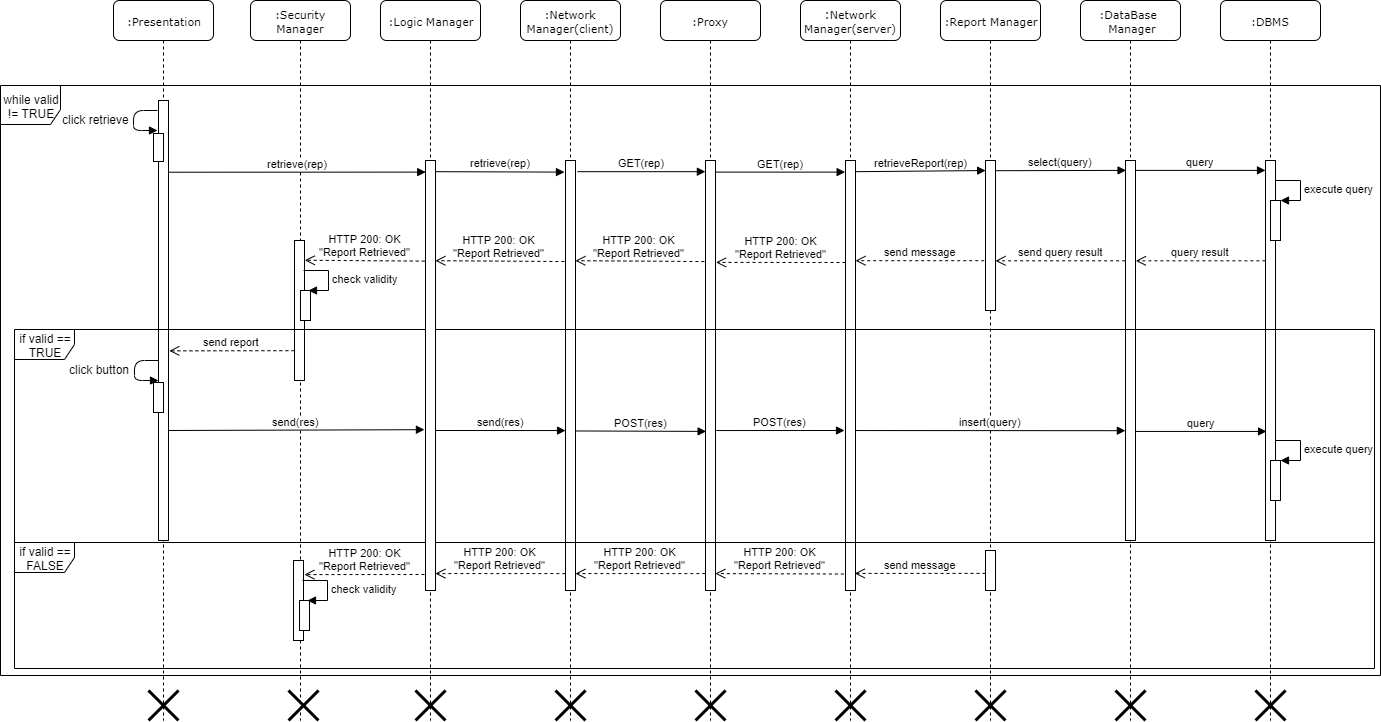
\includegraphics[scale=0.3]{img/sequence_diagrams/retrieve_report.png}
    \caption{Retrieve Report Runtime View}
\end{figure}  
\clearpage
\textbf{Retrieve Statistics Runtime View}\\
The following diagram describes the sequence of events when a \textit{User} tries to retrieve statistics in
\textit{SafeStreets} application. The actors involved are the Presentation, GPS, Google Maps, Logic Manager and 
the Network Manager on the client and the Network Manager, Statistics Manager and the Cache on the Server.
When a \textit{User} clicks the retrieve button two HTTP requests are sent, one to GPS Service and the other
one to Google Maps Service, in order to know the exact position of the \textit{User} and the area in which he is
using the app. After that an other HTTP request is sent to Application Server in order to retrieve statistics by 
quering DB. 
\\
\\
\\
\\
\\
\begin{figure}[H]
    \centering
    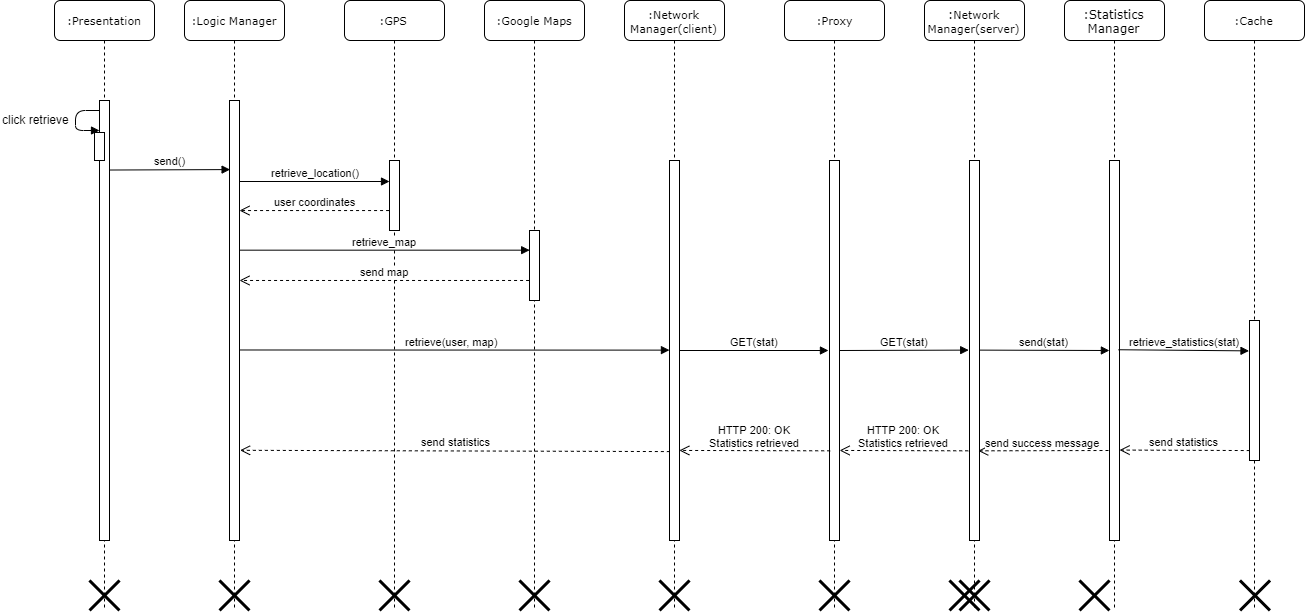
\includegraphics[scale=0.3]{img/sequence_diagrams/retrieve_statistics.png}
    \caption{Retrieve Statistics Runtime View}
\end{figure}  
\clearpage
\subsection{Component Interfaces}

Below are showed three picture representing the component interfaces diagram, the first is for client, the second
for server and the third is the complete diagram with all the components. Again we divided the perspective
of the image for the sake of readability.

\begin{figure}[H]
    \centering
    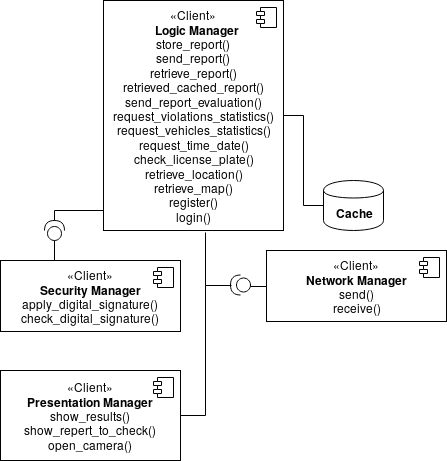
\includegraphics[scale=0.5]{img/component_interface_diagrams/client_component_interface.png}
    \caption{Client Component Interface Diagram}
\end{figure}
\begin{figure}[H]
    \centering
    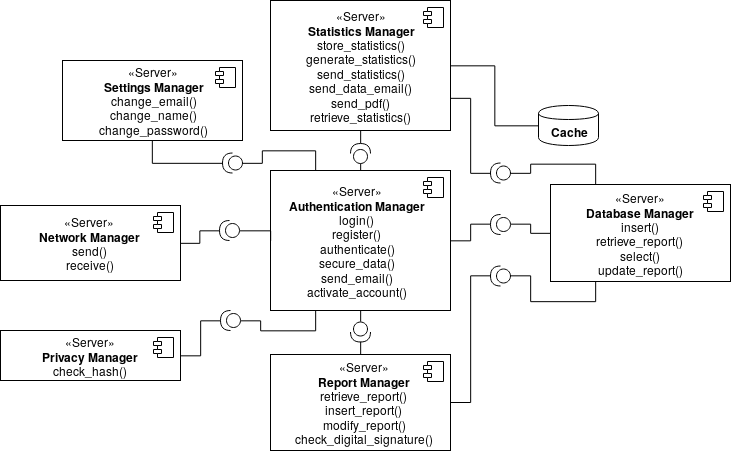
\includegraphics[scale=0.5]{img/component_interface_diagrams/server_component_interface.png}
    \caption{Server Component Interface Diagram}
\end{figure}
\begin{figure}[H]
    \centering
    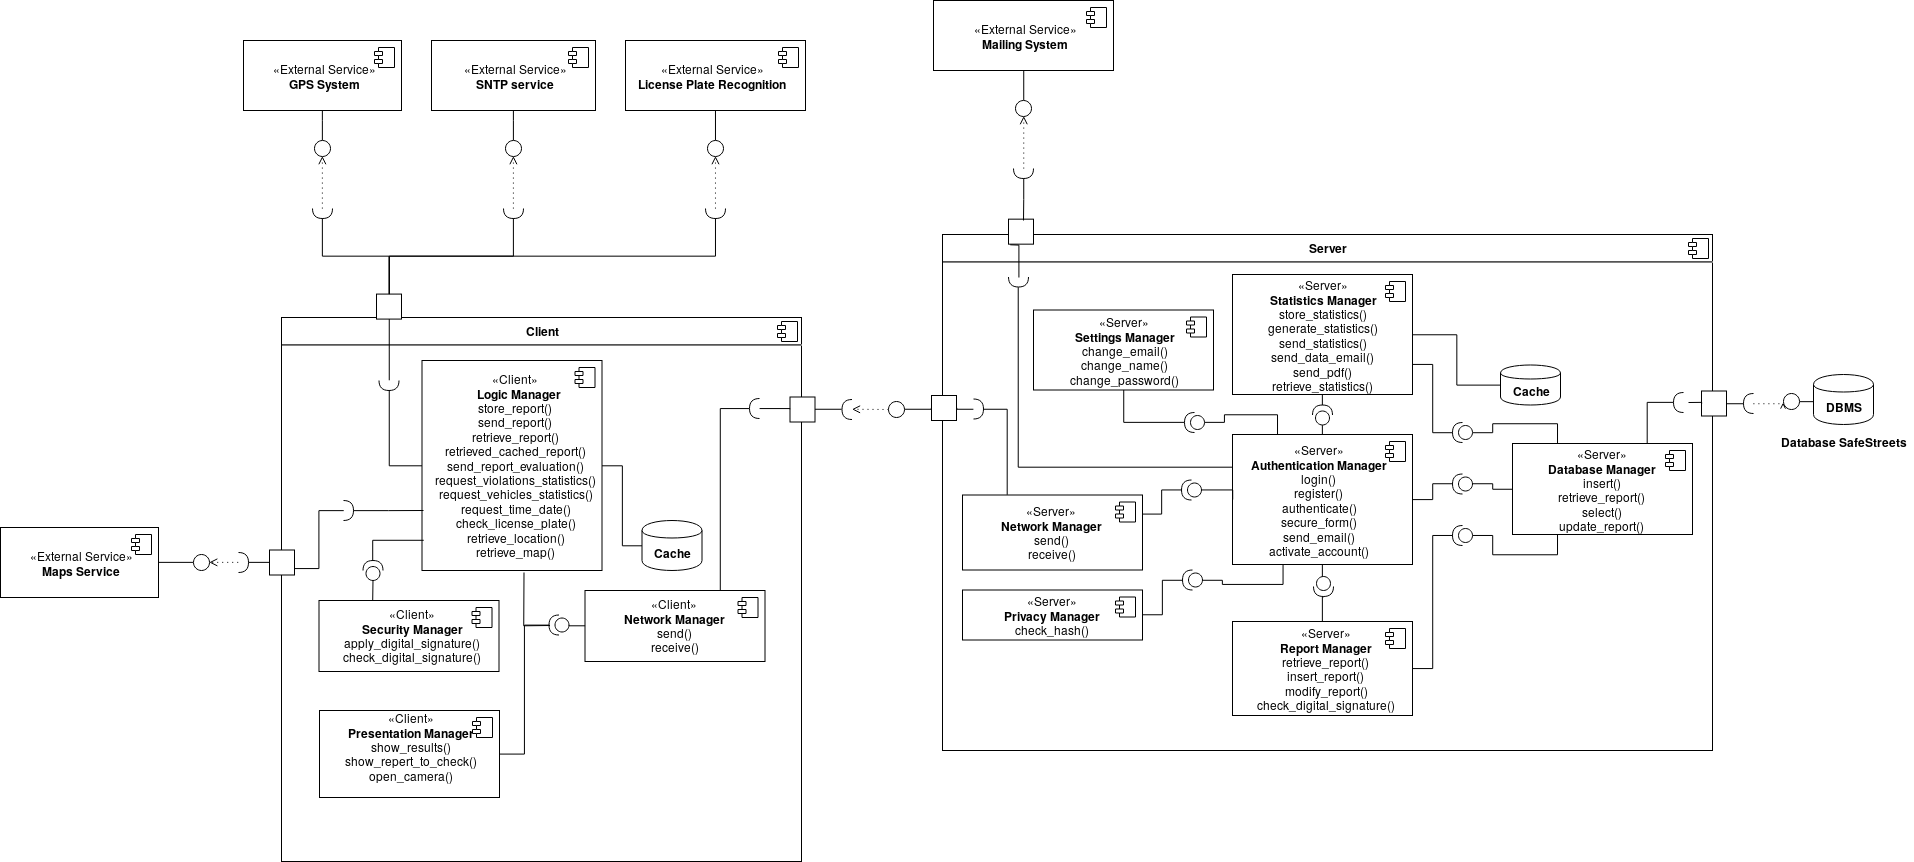
\includegraphics[width=1.2\textwidth, left]{img/component_interface_diagrams/component_interface.png}
    \caption{Component Interface Diagram}
\end{figure}

\clearpage

\subsection{Selected Architectural Style And Patterns}
\textbf{SafeStreets Architecture} \\
The architecture chosen for \textit{SafeStreets} is multi-tier, namely a 3-tier architecture. 
This choice is weighted based on the requirements that the \textit{System} must fulfill trying 
to optimize infrastructure costs at the same time. The tiers are divided into Client, 
Server and Database. The Client allows \textit{Users} to interact with \textit{SafeStreets}, takes care of 
the presentation, the digital signature, the exchange of messages with the server and the 
generation of the report. The logic in the client concerns only the temporary caching of 
the report and a possible resubmission in the case of a malicious attack on the report 
(both in the case of the \textit{Citizen} to avoid loss in case of error and for the \textit{Authority} 
that must evaluate it), collecting data from various external services and securing the 
report during trasmission to server. \\From these premises and considering that all the other 
operations, such as the generation of the statistics or the update of these are made, 
necessarily, on the server side, the client is to be considered a thin client. 
The Server on the other hand will have a greater workload, the chosen architecture is 
NginX, which has a more flexible architectural design than the Apache process-driven one. 
Furthermore NginX is much more efficient than apache in presenting static content, 
this is in favor of \textit{SafeStreets} since the statistics, which may seems dynamic, 
actually arrive to the \textit{User} in the form of static content. This is because, as 
the \textit{SafeStreets} logic was designed, the statistics are updated only thanks to the 
control of an \textit{Authority}, this implies that the process of updating the statistics 
is not very fast, and that these can be generated at regular time intervals saving 
them in cache and sending them to the clients in static form. This brings great 
advantages to the application in terms of workload and service speed.\\ In fact, 
generating statistics at each client-side request would be unsustainable, so the 
server-side load is drastically reduced. In order to have greater \textit{System} portability and 
scalability in case of required memory space growth, the best choice for the database is 
entrusting to an external service. This choice not only saves on costs, maintenance and 
the skills required but also guarantees a remarkable scalability in performance.
\\
\\
\textbf{REST} \\
Our \textit{System} uses the REpresentational State Transfer (REST) architectural style. This 
approach brings great advantages in terms of scalability and more, future changes to the software 
or additional features will not be a problem as thanks to the API it will be easy to add features 
without creating problems to existing ones. Furthermore, this approach also brings great improvements 
in tolerance to changes and failures. HTTP is the communication protocol used underneath, 
so CRUD operations are implemented through GET, POST, DELETE and PUT primitives. 
\\
\\
\textbf{Patterns}\\
In the following paragraph will be described the design patterns used in \textit{SafeStreets}. 
\\
\\
\textbf{MVC}\\
Our \textit{System} follows the MVC paradigm. The acronyms stands for Model View Controller

\begin{itemize}
    \item The Model corresponds to the component containing all the application's data and integrity constraints. 
    In our case the Model is described in the external database.
    \item The View corresponds to the presentation layer, the client's only interface with the \textit{System}.
    \item The Controller is responsible for the logic of the application and in our case corresponds to \textit{SafeStreets}'s Server.
\end{itemize}
\textbf{Visitors Pattern}\\
Both Network Manager client and server side will adopt this patter in order to route correctly the messages. \textit{SafeStreets}
router logic is embedded in The Network Manager, this choice aims to simplify the sending of a message to a component
from another. It will be easy and flexible to add new type of message and, adding a new component, we only needs to 
add it on the Network Manager.
\\
\\
\textbf{Adapter Pattern}\\
In order to separate interfaces from main logic we need to use this pattern. This separation is necessary to guarantee
scalability and to simplify future improvements.

\clearpage

\subsection{Other design decision}
\textbf{Firewall}\\
Our \textit{System} use two firewalls to create a DMZ. The first 
firewall must be configured to allow traffic destined to the DMZ only. The second firewall only 
allows traffic to the DMZ from the internal network. This setup is considered more secure since two 
devices would need to be compromised. Network firewalls operate by filtering the packets trying to 
pass through them.
\\ 
\\
\textbf{DataBase}\\
It was decided to use a relational database model for \textit{SafeStreets}, as opposed to a 
non-relational model, because it allows to represent the intrinsic relationships present in 
the data needed to be stored. Also, many complex operations will be made on the database, 
including Joins and Updates, which are not well handled by a non-relational model. The database will use
an ORM to simplify the interaction with Managers. Also the Database is acquired on premise as 
an external service.
\\ 
\\
\textbf{ER Diagram}\\
This is an oversimplified representation of the database schema. This is only a general view 
on the mandatory attributes needed focusing on the relevant attributes and tables. We omitted 
for simplicity other attribute less important, statistics for example may need some other attributes 
useful to perform searches more efficiently. In the ER schema there are five main entities:  
\textit{Citizen} and \textit{Authority} identified as \textit{Users}, the two entity Vehicle and 
Location separated in two distinct table in order to make the process of statistics generation more 
efficient as possible and the entity Violation that is identified by date, time, location and license 
plate to guarantee unicity. 

\begin{figure}[H]
    \centering
    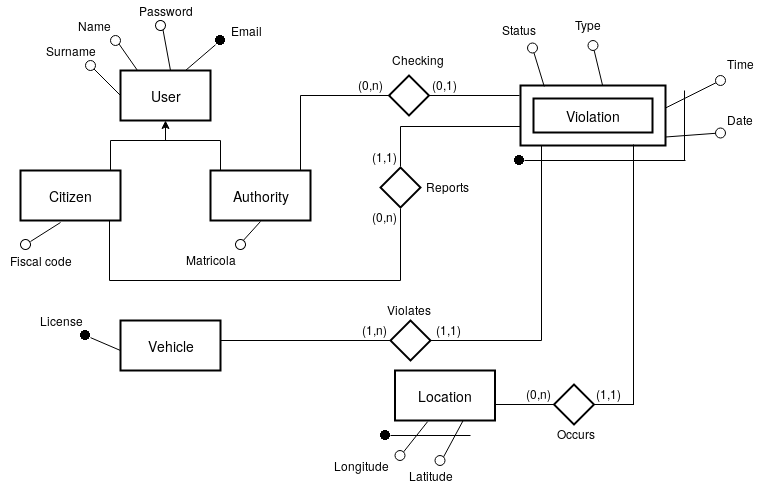
\includegraphics[scale=0.5]{img/ER_diagram.png}
    \caption{ER Diagram}
\end{figure}

\clearpage

%%%%%%%%CHAPTER 3%%%%%%%%%%%%

\section{User Interface Design}
Since the mockups are described in the RASD, in this section the focus is only on the UI flow i.e. on how
those mockups are linked, and how \textit{Users} can navigate through them.
\\
This is the application main flow either for the \textit{Citizen} and \textit{Authority}, they both start with login 
or registration and then they have access to the respective pages. \textit{Citizen} will be able to 
visualize violations statistics, settings and send report page. The \textit{Authority} can access 
same statistics as \textit{Citizen} plus vehicles statistics and the page in which can retrieve report 
information and also a settings page.

\begin{figure}[H]
    \centering
    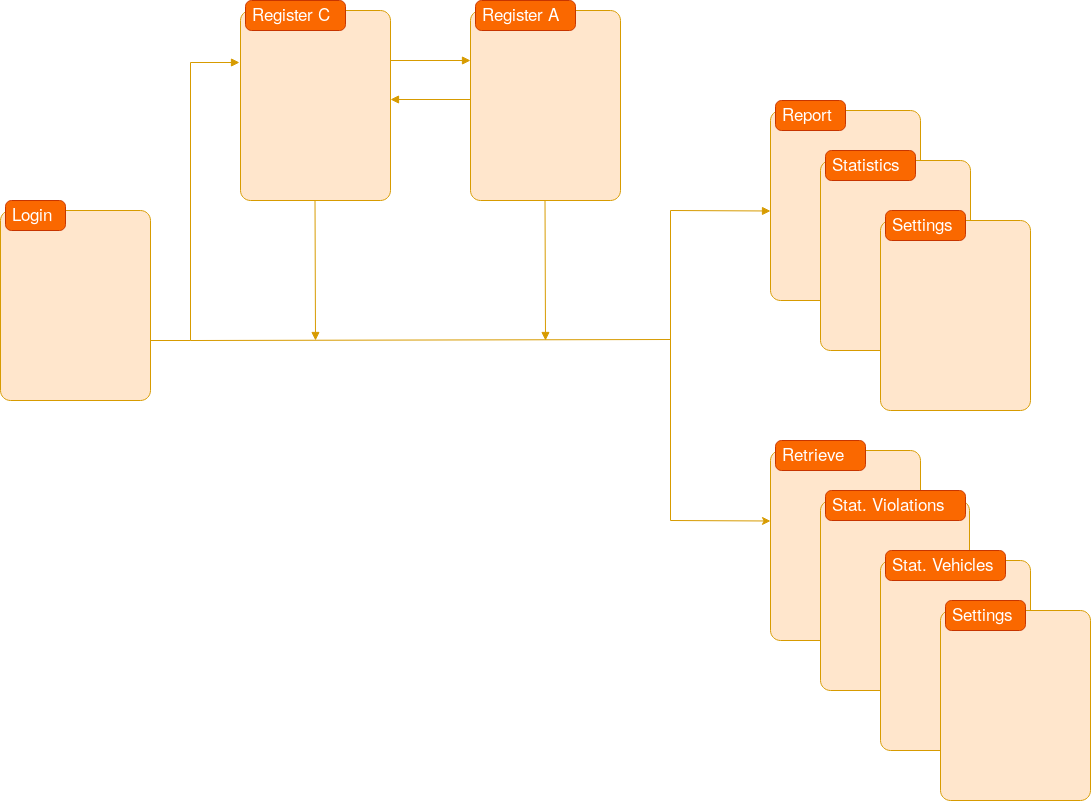
\includegraphics[scale=0.3]{img/UX_flow.png}
    \caption{UI flow}
\end{figure}

%%%%%%%%!CHAPTER 3%%%%%%%%%%%%

\section{Requirements Traceability}
\begin{center}
    \begin{tabular}{ | l | l |}
        \hline
        COMPONENT(DD) & REQUIREMENTS(RASD) \\
        \hline
        Authentication Manager & \textbf{[R1]}: Account can be created if and only if \textit{User} provides unique \\ 
                               & email and password \\
                               & \textbf{[R2]}: The \textit{System} allows Guest to create \textit{Citizen} or \textit{Authority} account \\
        \hline
        Report Manager  & \textbf{[R14]}: The \textit{System} has to save the confirmed violation in the DB. \\
                        & \textbf{[R18]}: The violation retrieved can only be seen by the \textit{Authority} that \\
                        & retrieves it \\
                        
        \hline
        Statistics Manager & \textbf{[R12]}: \textit{Users} can change the area of visualization \\
                           & \textbf{[R13]}: \textit{Users} can change the date of visualization \\
                           & \textbf{[R15]}: \textit{Authority} can search for a specific license plate \\
                           & \textbf{[R19]}: The \textit{System} must update the statistics with the most recent data \\
        \hline
        Privacy Manager & \textbf{[R17]}: The \textit{System} must use HTTPS to safely communicate \\
        \hline 
        Settings Manager & \textbf{[R3]}: The \textit{System} allow \textit{User} to modify his settings. \\
        \hline
        DataBase Manager & \textbf{[R14]}: The \textit{System} has to save the confirmed violation in the DB. \\
        \hline
        Security Manager & \textbf{[R16]}: Violations sent must be digitally signed \\
                         & \textbf{[R17]}: The \textit{System} must use HTTPS to safely communicate \\
        \hline
        Logic Manager   & \textbf{[R1]}: Account can be created if and only if \textit{User} provides unique \\ 
                        & email and password \\
                        & \textbf{[R2]}: The \textit{System} allows Guest to create \textit{Citizen} or \textit{Authority} account \\
                        & \textbf{[R3]}: The \textit{System} allow \textit{User} to modify his settings. \\
                        & \textbf{[R4]}: The \textit{Citizen} has to take the violation’s photo with the application \\
                        & \textbf{[R5]}: The \textit{System} allows \textit{Citizen} to input some violation’s data \\
                        & \textbf{[R6]}: The photo taken must be recognizable by the \textit{System} \\
                        & \textbf{[R7]}: The \textit{Citizen} has to be able to discard the photo taken \\
                        & \textbf{[R8]}: The \textit{System} has to be able to attach the correct date, time and \\ 
                        & position to the report \\
                        & \textbf{[R9]}: The \textit{Citizen} can’t change date, time and position in the report \\ 
                        & \textbf{[R10]}: \textit{Citizen} can change the license plate if it isn’t recognised properly \\
                        & \textbf{[R11]}: \textit{Citizen} has to be able to choose the correct type of violation \\
                        & \textbf{[R16]}: Violations sent must be digitally signed \\
        \hline
    \end{tabular}
    \end{center}
%%%%%%%%%% !CAHPTER 4 %%%%%%%%%%
\clearpage
%%%%%%%%%% CHAPTER 5 %%%%%%%%%%
\section{Implementation, Integration and Test Plan}
Regarding the implementation and testing, the approach chosen is Agile, much more flexible 
than the old Waterfall approach, in order to allow us to bring to the user a working software 
and above all a software that is durable and flexible to changes.

\subsection{Overview}
For what concern the part of implementation we identify 3 macros subsystems:
\begin{itemize}
    \item The client subsystem, containing the presentation.
    \item The server subsystem, containing components of Server and the interaction with DB.
    \item External Services, such as DB, Maps Service, STNP Service, License Plate Recognition Service. 
\end{itemize}  
Our implementation and testing will be incremental and will follow the bottom-up approach.

\subsection{Implementation}
The order of implementation we decided to follow is necessary in order to obtain consistency:
\begin{enumerate}
    \item creation of the Database and its costraints.
    \item server and client implementation
    \item integration with external services
\end{enumerate}
The implementation of the server and the client will be in parallel in order to increase the efficiency.
The implementation of the server will follow this order:
\begin{enumerate}
    \item Database manger
    \item Network manager 
    \item Authentication manager 
    \item Privacy manager
    \item Settings manager
    \item Report manager
    \item Statistics manager
\end{enumerate}
In particular DataBase Manager and Network Manager will be implemented first because they represents the access 
point to the Clients and the DB. 
\\
\\
For what concern the implementation of the client:
\begin{enumerate}
    \item \textit{User} Interface implementation
    \item Network manager
    \item Presentation manager
    \item Security manager
    \item Logic manager
\end{enumerate}
\subsection{Unit testing}
During the whole phase of implementation component's unit tests will be performed in order to find any possible kind of bugs.
Unit tests will be added incrementally as new code is written. In this way is possible to fix bugs with the lowest cost of 
repair in terms of effort and time. Using the bottom-up approach we need to simulate the components that are missing in order
to test the component just added. To do so driver will be used to simulate calls to a certain component. Stubs, instead, will be 
used to simulate external services such as Maps Service or STNP service.    


\subsection{Integration testing}
In this section we will show how components will be integrated. The arrows start from the component which ‘uses’ the other one. 
\\
\\
\textbf{Integration of internal components of the Application Server}
\begin{figure}[H]
    \centering
    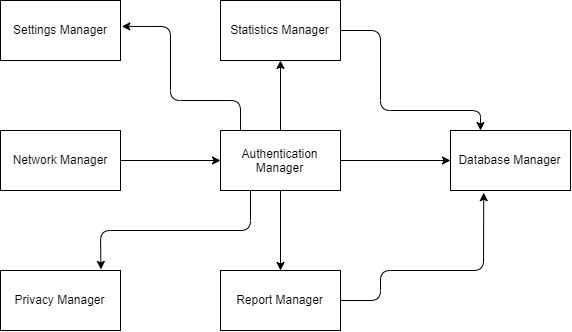
\includegraphics[scale=0.5]{img/integration/Server_test.png}
    \caption{Server Integration}
\end{figure}

\textbf{Integration of Client}
\begin{figure}[H]
    \centering
    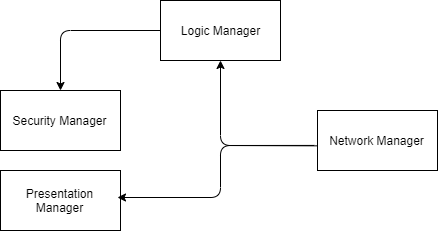
\includegraphics[scale=0.5]{img/integration/Client_test.png}
    \caption{Client Integration}
\end{figure}

\textbf{Integration of Client-Server}
\begin{figure}[H]
    \centering
    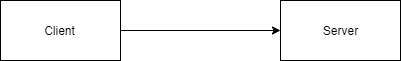
\includegraphics[scale=0.5]{img/integration/ClientServer_test.png}
    \caption{Client Server Integration}
\end{figure}

\textbf{Integration of External Services}
\begin{figure}[H]
    \centering
    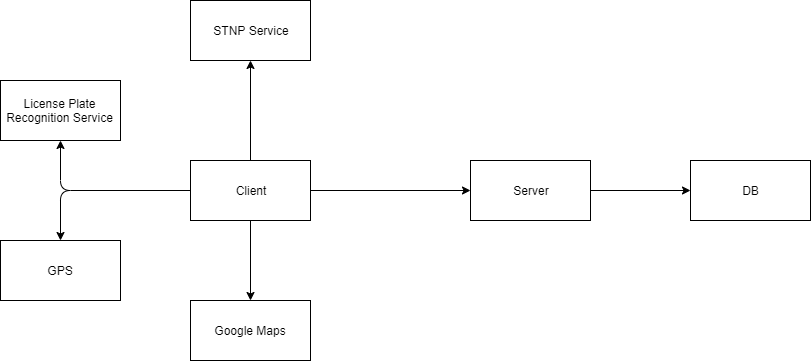
\includegraphics[scale=0.4]{img/integration/ExternalService_test.png}
    \caption{External Service Integration}
\end{figure}

\clearpage

\section{Efforts}

\begin{center}
\begin{tabular}{ | l | l | l |}
    \hline
    Efforts & Dario & Pierriccardo \\
    \hline
    initial setup & 1h & 1h \\
    \hline
    chapter 1 & 1h & 2h \\
    \hline
    chapter 2 & 40h & 42h \\
    \hline
    chapter 3 & 1h & 2h \\
    \hline
    chapter 4 & 3h & 1h \\
    \hline
    chapther 5 & 3h & 2h \\ 
    \hline
    group work & 20h & 20h \\
    \hline
    total & 69h & 71h \\
    \hline
\end{tabular}
\end{center}
\end{document}